
\clearpage
\section{Eigenfunctions of a one-dimensional overlapping grid problem}\label{sec:eigenfunctions}

\input \ogmgDocDir/compositeGrid1D.tex

  The multigrid algorithm is based on the ability of smoothers to reduce the errors in the
high-frequency components of the solution and of the coarse grid to represent the smooth components.
It can be instructive to study the structure of the eigenfunctions to the Laplace operator
on an overlapping grid. In this section we consider a one dimensional overlapping grid and determine the
eigenfunctions to the Laplace operator.






In one-dimension we consider solutions to the eigenvalue problem
\begin{align*}
    u_{xx} &= \lambda u  \qquad \xv\in\Omega=(x_a,x_b) \\
    u &= 0  \qquad \xv\in\partial\Omega
\end{align*}
We discretize this problem on a one-dimensional overlapping grid, shown in figure~(\ref{fig:overlappingGrid1D}),
with discrete approximation given by
\begin{align*}
   U_0 &= 0 \\
   D_{+1}D_{-1} U_i = (U_{i-1}-2U_i + U_{i+1}) h_1^{-2} & = \lambda U_i \qquad i=2,3,\ldots,N_1-1 \\
   U_{N_1} &= \sum_{m=0}^M \alpha_m V_{p+m} \qquad \mbox{(interpolation)}\\
   V_0 &= \sum_{m=0}^M \beta_m U_{q+m} \qquad \mbox{(interpolation)}\\
   D_{+2}D_{-2} V_i = (V_{i-1}-2V_i + V_{i+1}) h_2^{-2}  & = \lambda V_i \qquad i=2,3,\ldots,N_2-1 \\
   V_{N_2} &=0 
\end{align*}
Here $U_i\approx u(x_{1i})$, $x_{1i}=x_a+i h_1$ denotes the solution on the interval $[x_a,x_d]$
and $V_i\approx u(x_{2i})$, $x_{2i}=x_c+i h_2$ denotes the solution on the interval $[x_c,x_b]$.

For linear interpolation (M=2) we use
\begin{align*}
  U_m &= (1-\alpha) V_p + \alpha V_{p+1} \\
  V_0 &= (1-\beta) U_q + \beta U_{q+1} 
\end{align*}
where 
\begin{align*}
     p&=   \lfloor (x_d-x_c )/h_2 \rfloor \qquad\mbox{($ \lfloor x \rfloor$ is the greatest integer less than $x$)}\\
  \alpha &= (x_d-x_c )/h_2 - p \\
     q&=   \lfloor (x_c-x_a )/h_1 \rfloor \\
  \beta  &= (x_c-x_a )/h_1 - q 
\end{align*}
For quadratic interpolation (M=3) we use
\begin{align*}
  U_m &= \alpha_0 V_p + \alpha_1 V_{p+1} + \alpha_2 V_{p+2} \\
  V_0 &= \beta_0 U_q + \beta_1 U_{q+1} +\beta_2 U_{q+2}
\end{align*}
Quadratic interpolation is normally required for second-order accuracy.

Figure~(\ref{fig:eig1d-a}) shows the eigenfunctions for 3 different values of the
overlap width, $d=x_d-x_c$. The eigenfunctions have been shifted in the vertical direction for clarity.
When the overlap width is $d=1$ the problem reduces to that of a single non-overlapping grid for
the entire interval $[x_a,x_b]$. In the case when the overlap width is small, $d\approx .5h$, 
the eigenfunctions are nearly the same as the single grid case. When the overlap width is large,
there are some eigenfunctions that do not look like those from the single grid, see eigenfunction number $9$...

\renewcommand{\figWidth}{.45\linewidth}
\begin{figure}
\begin{center}
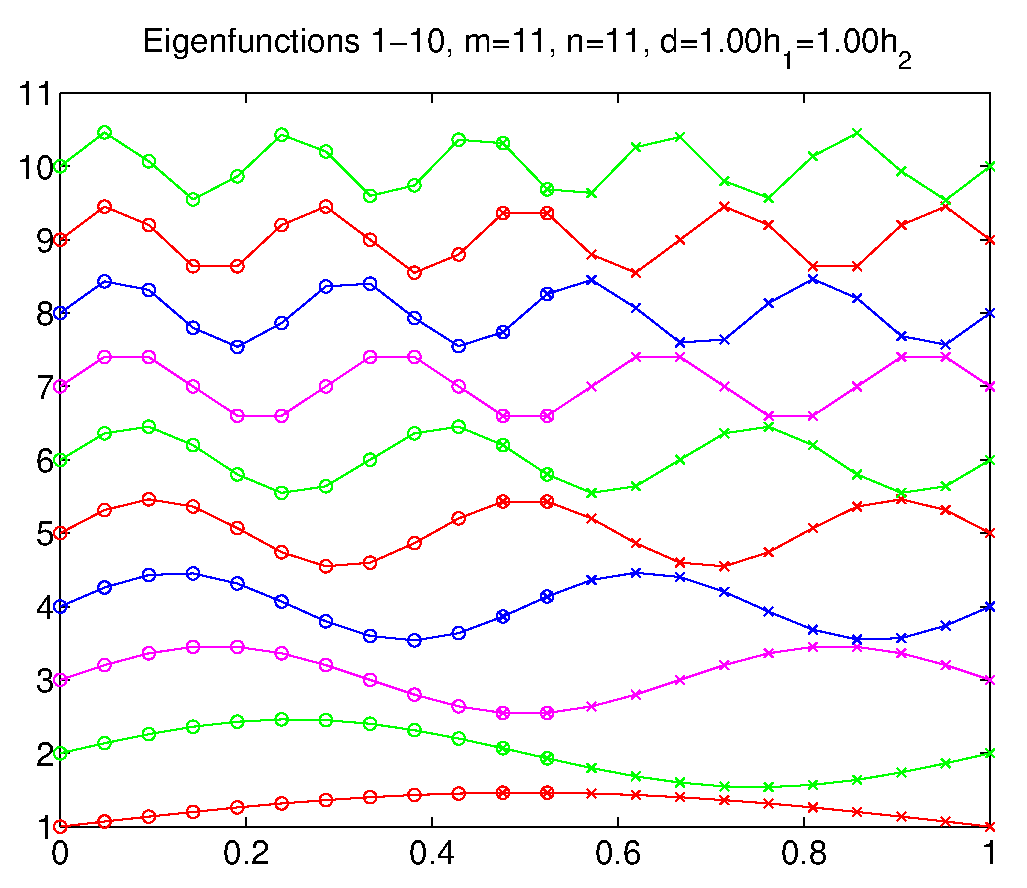
\epsfig{file=\ogmgDir/eigenfunction-d1p0-1.eps,width=\figWidth}
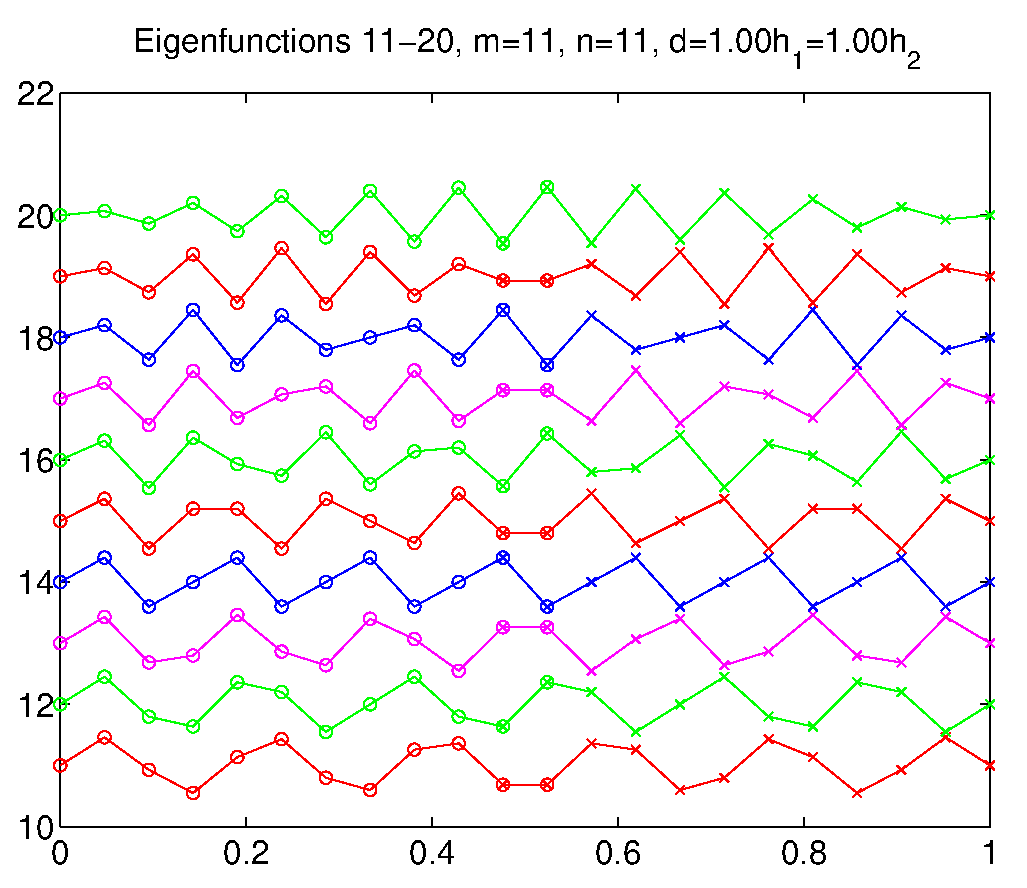
\epsfig{file=\ogmgDir/eigenfunction-d1p0-2.eps,width=\figWidth}
\vskip\baselineskip
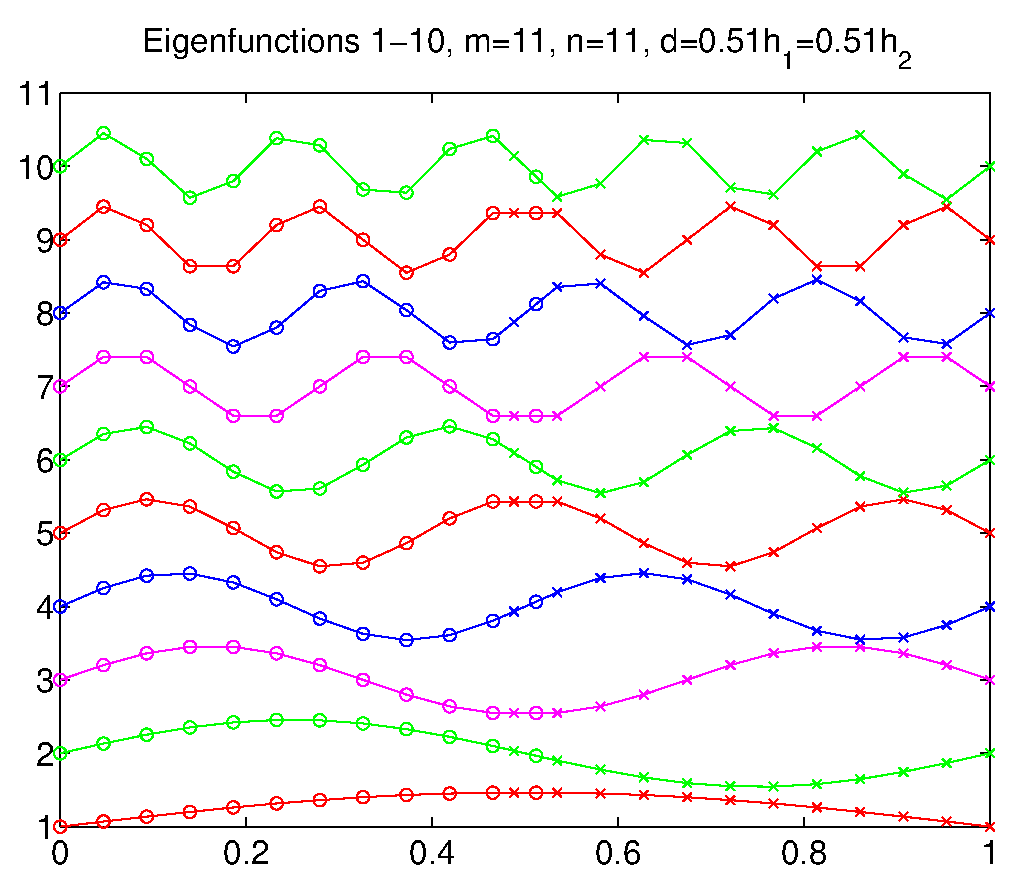
\epsfig{file=\ogmgDir/eigenfunction-dp5-1.eps,width=\figWidth}
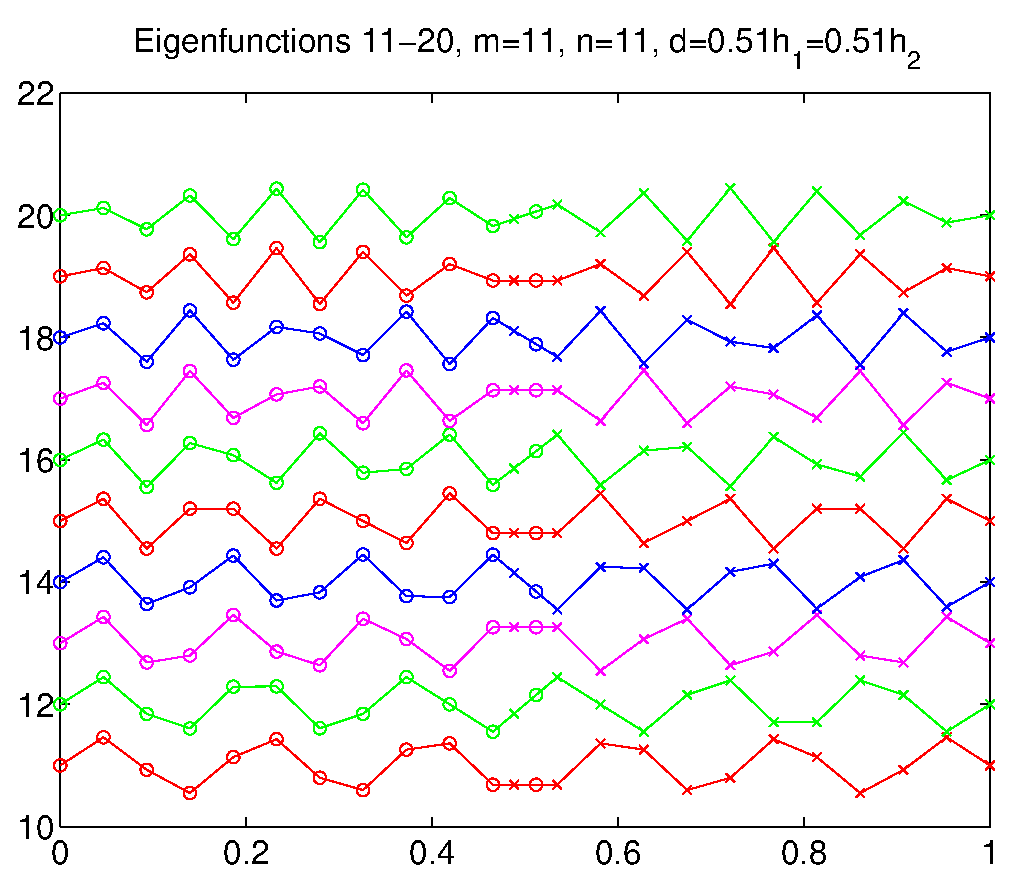
\epsfig{file=\ogmgDir/eigenfunction-dp5-2.eps,width=\figWidth}
\vskip\baselineskip
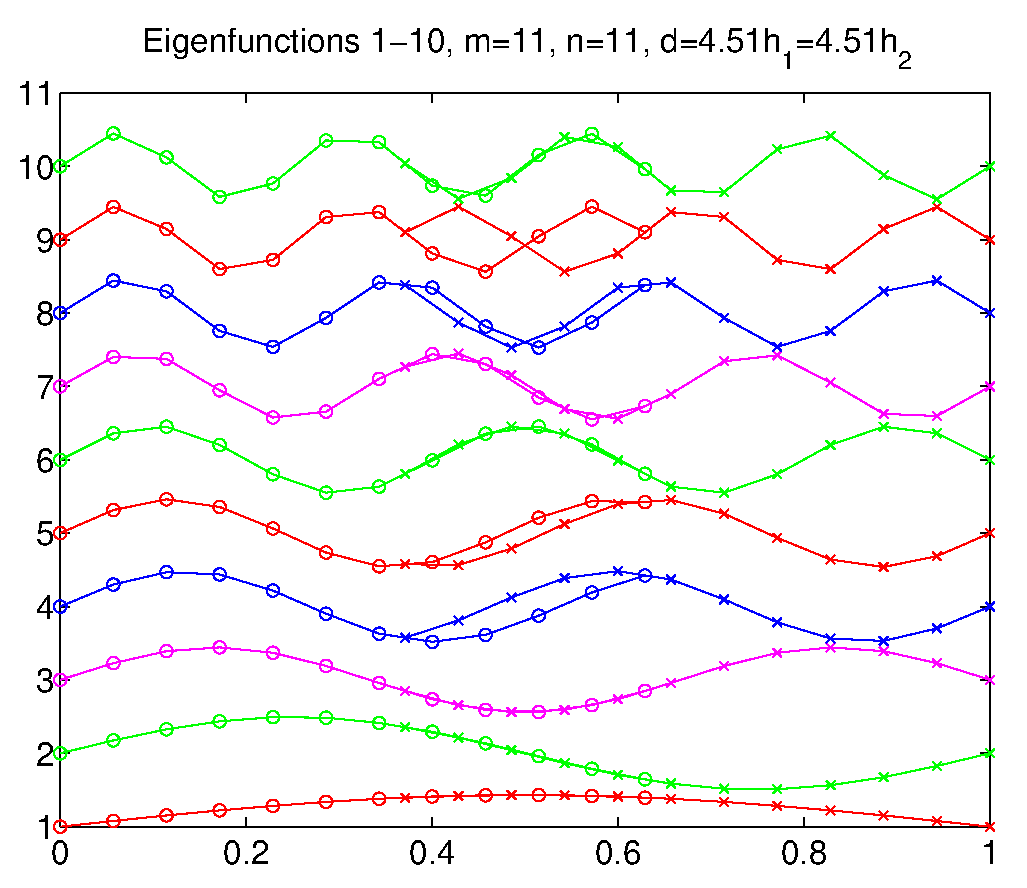
\epsfig{file=\ogmgDir/eigenfunction-d2p75-1.eps,width=\figWidth}
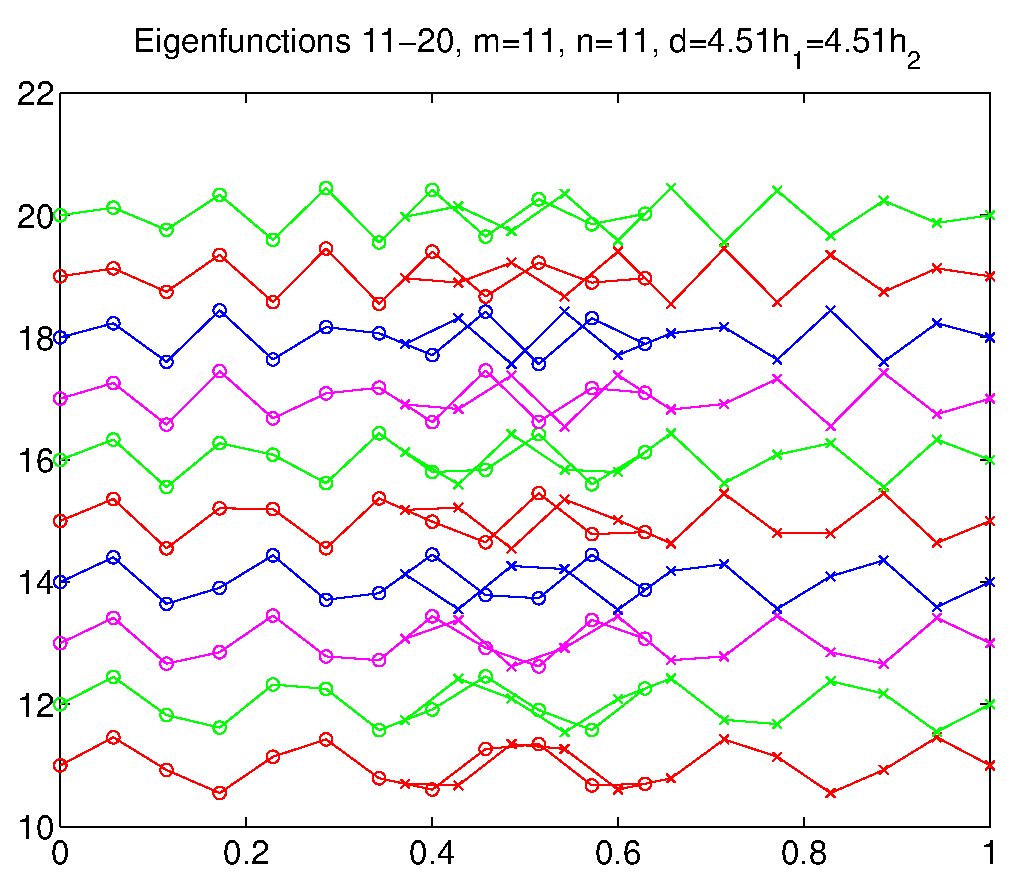
\epsfig{file=\ogmgDir/eigenfunction-d2p75-2.eps,width=\figWidth}
\end{center}
\caption{Eigenfunctions to the Laplace operator on a one-dimensional overlapping grid, $N_1=11$, $N_2=11$.
  Top $d=h$ (equivalent to a single grid). Middle: $d=.51h$. Bottom: $d=4.51h$. }
\label{fig:eig1d-a}
\end{figure}

\begin{figure}
\begin{center}
% \epsfig{file=\ogmgDir/eigenfunction17-5-d1p0-1.eps,width=\figWidth}
% \epsfig{file=\ogmgDir/eigenfunction17-5-d1p0-2.eps,width=\figWidth}
\vskip\baselineskip
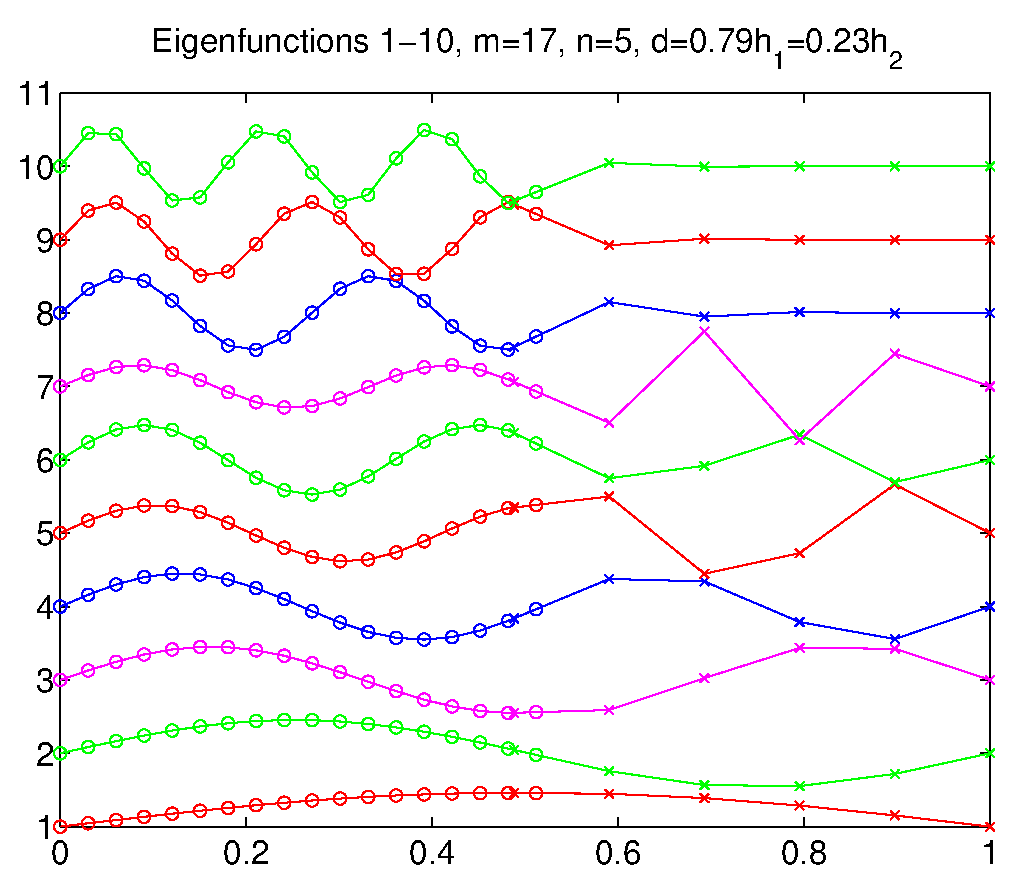
\epsfig{file=\ogmgDir/eigenfunction17-5-dp5-1.eps,width=\figWidth}
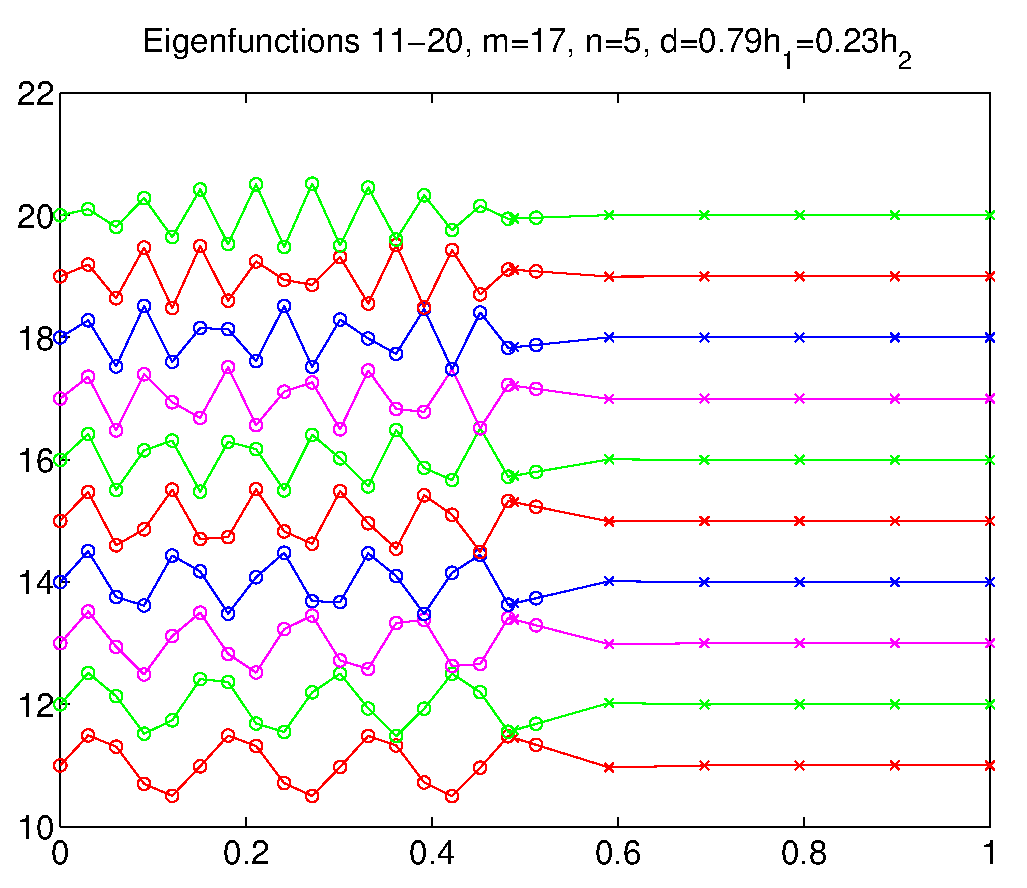
\epsfig{file=\ogmgDir/eigenfunction17-5-dp5-2.eps,width=\figWidth}
\vskip\baselineskip
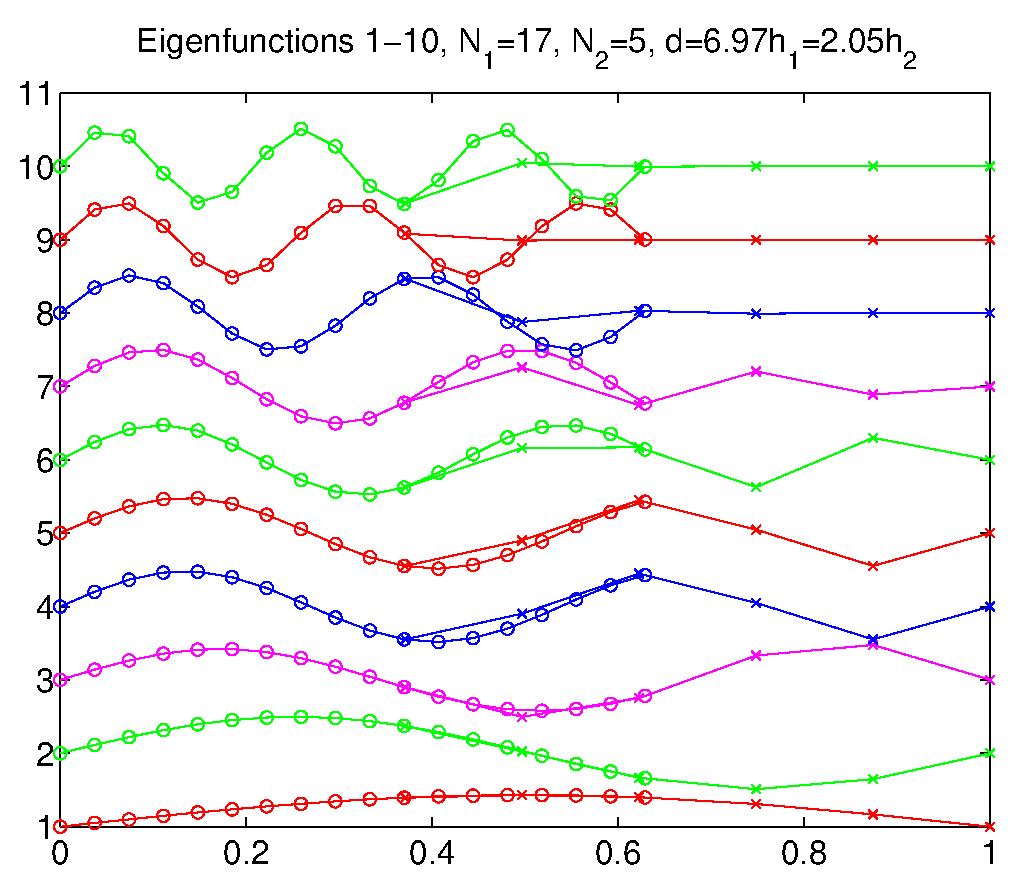
\epsfig{file=\ogmgDir/eigenfunction17-5-d2p75-1.eps,width=\figWidth}
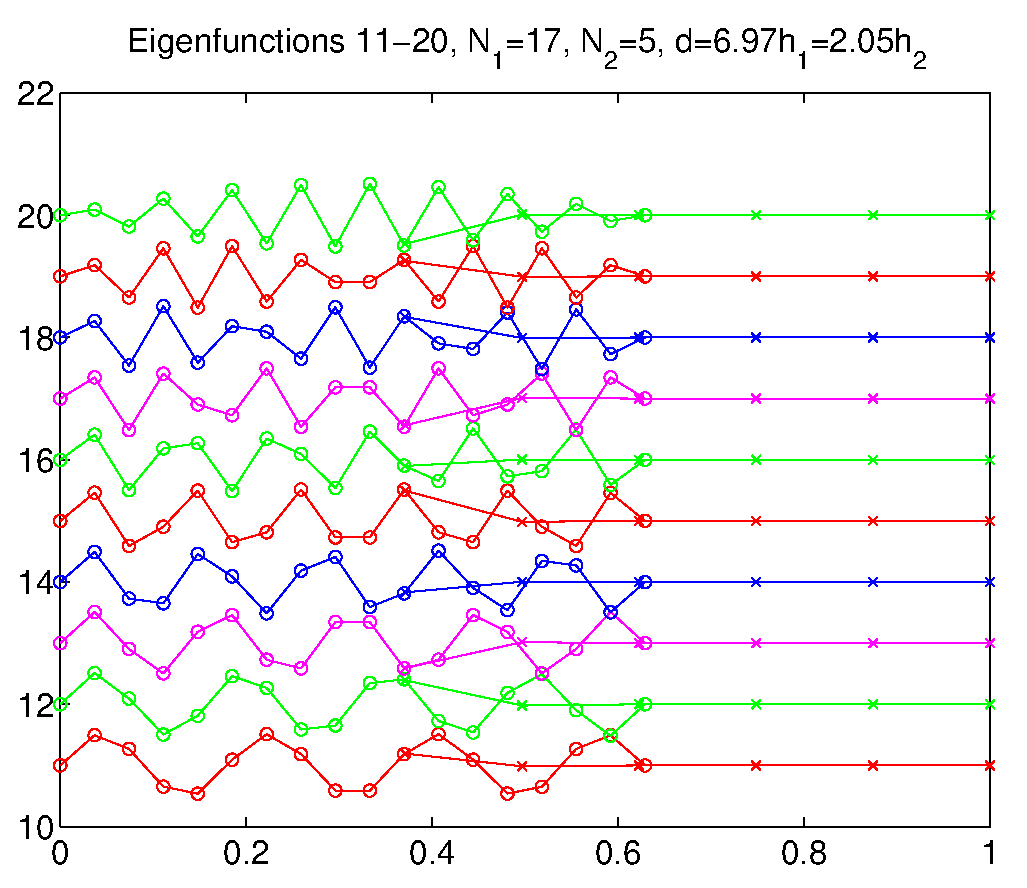
\epsfig{file=\ogmgDir/eigenfunction17-5-d2p75-2.eps,width=\figWidth}
\end{center}
\caption{Eigenfunctions to the Laplace operator on a one-dimensional overlapping grid, $N_1=17$, $N_2=5$.
  Top $d=??h$. Middle: $d=??h$. Bottom: $d=??h$. }
\label{fig:eig1d-b}
\end{figure}



% \begin{figure}
% 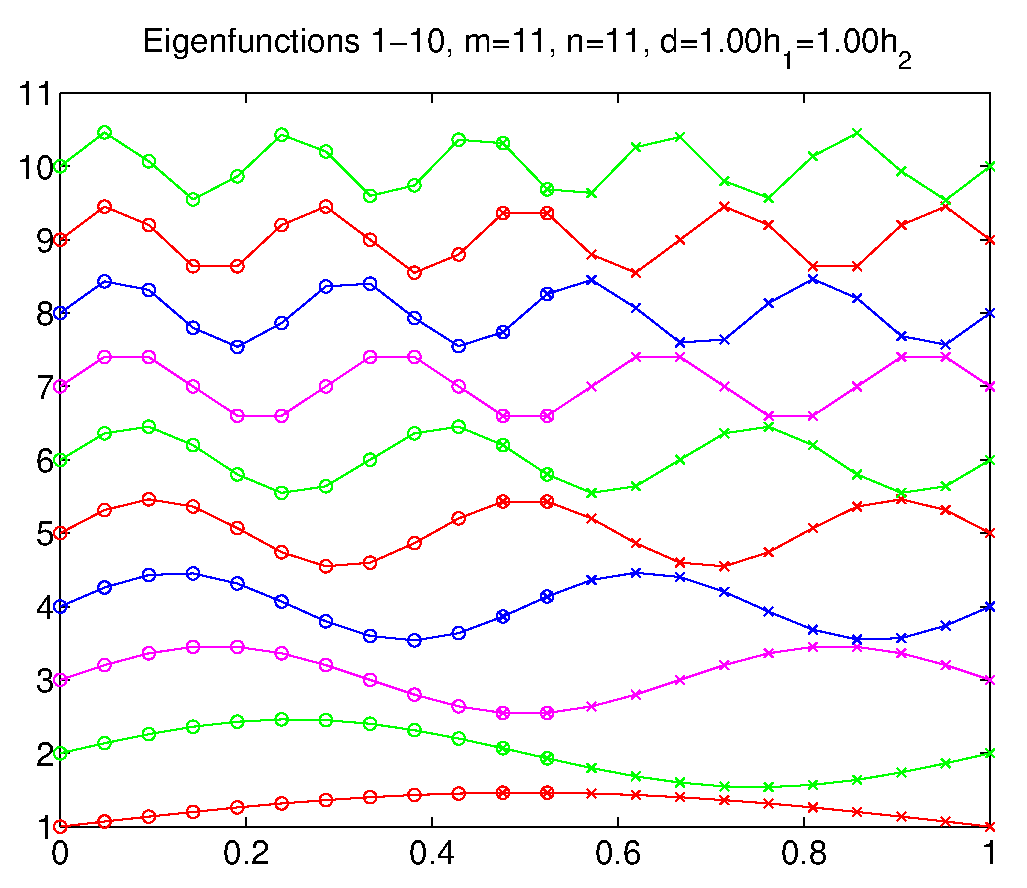
\epsfig{file=\ogmgDir/eigenfunction-d1p0-1.eps,width=\figWidth}
% 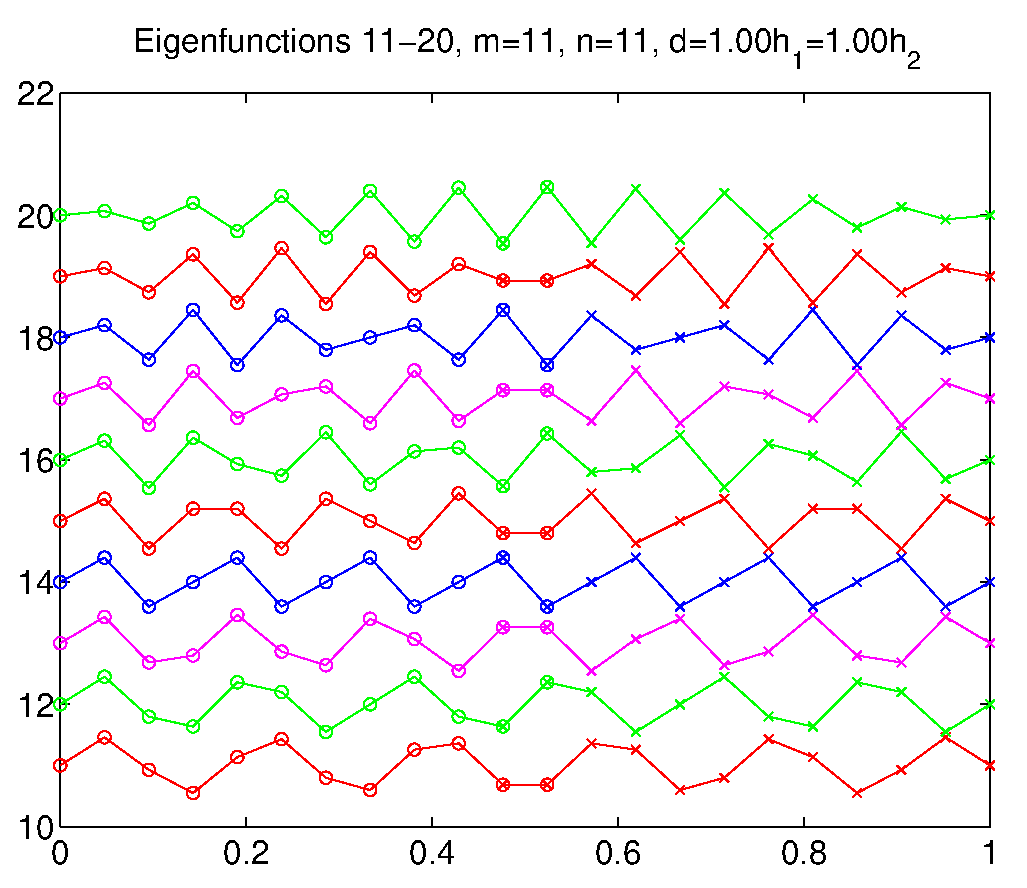
\epsfig{file=\ogmgDir/eigenfunction-d1p0-2.eps,width=\figWidth}
% \begin{center}
% end{center}
% \caption{Eigenfunctions to the Laplace operator on a one-dimensional overlapping grid, $d=h$. In this case
%    the eigenfunctions reduce to those of a single grid with no overlap.}
% \label{fig:eig1d}
% \end{figure}
% 
% \begin{figure}
% \begin{center}
% 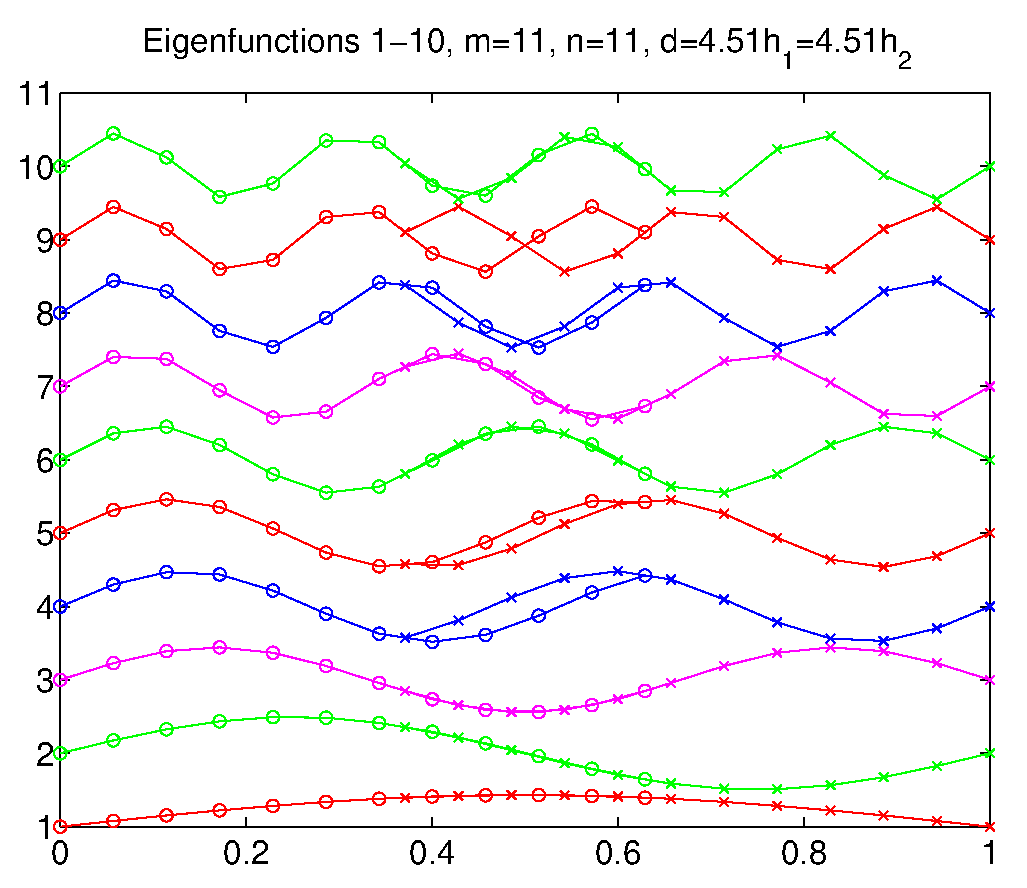
\epsfig{file=\ogmgDir/eigenfunction-d2p75-1.eps,width=\figWidth}
% 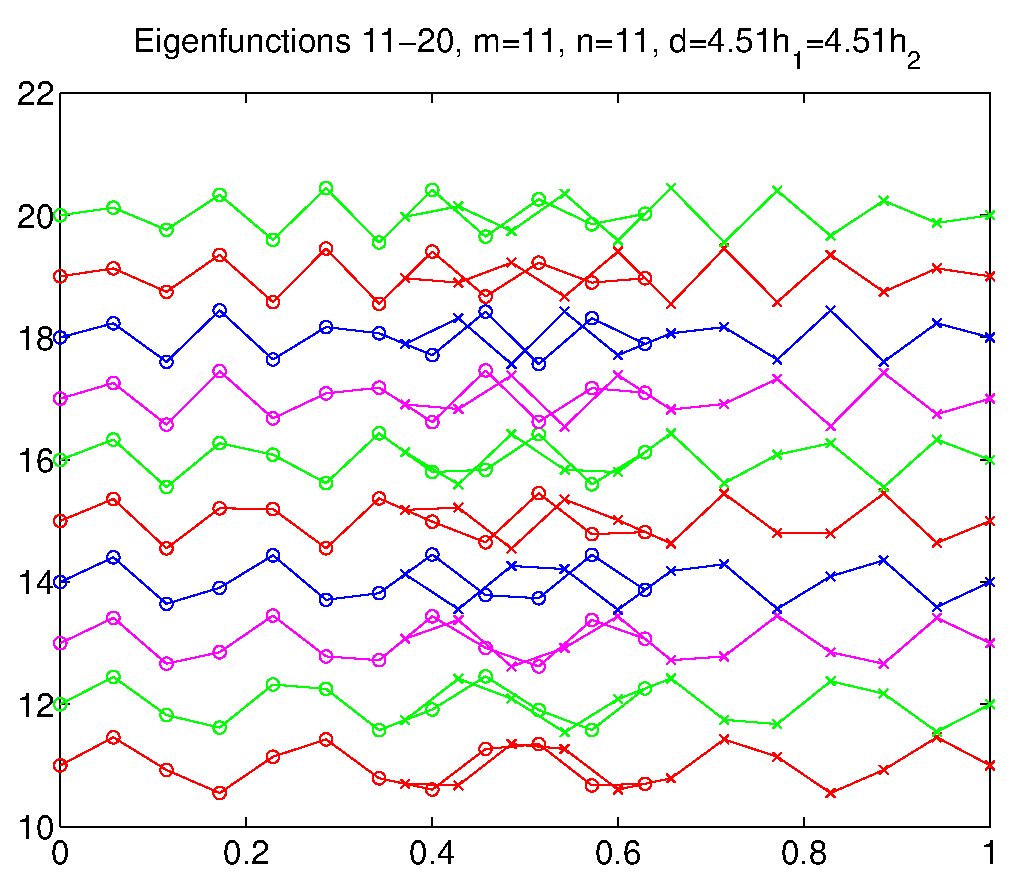
\epsfig{file=\ogmgDir/eigenfunction-d2p75-2.eps,width=\figWidth}
% \end{center}
% \caption{Eigenfunctions to the Laplace operator on a one-dimensional overlapping grid, $d=2.75h$.}
% \label{fig:eig1d}
% \end{figure}


\clearpage
\section{Overlap versus no overlap}

In this section we compare results for a square when the overlapping grid
consists of a single grid or two grids.

Table~(\ref{tab:overlap}) shows the results for a number of cases. The convergence rate depends
to some degree on the overlap distance between the grids. When the overlap distance is $d=1.$,
the convergence rates for the two-grid case are nearly the same as for the single grid.
When the overlap distance is the minimum value that we usually allow, $d=.5$, the convergence rate
is degraded somewhat but still quite good. Better results for $d=.5$ are obtained for a smaller
value of the over-relaxation parameter.

\renewcommand{\tablefontsize}{\footnotesize}
\begin{table}[hbt]
\begin{center}{\tablefontsize
\begin{tabular}{|c|c|c|c|c|} \hline 
 $i$   & res      & rate    &  WU    & ECR  \\   \hline 
 $ 1$  & $ 1.3e+03$ & $0.024$ & $ 5.0$ & $0.48$ \\ 
 $ 2$  & $ 1.1e+01$ & $0.008$ & $ 5.0$ & $0.38$ \\ 
 $ 3$  & $ 1.8e-01$ & $0.017$ & $ 5.0$ & $0.44$ \\ 
 $ 4$  & $ 2.8e-03$ & $0.015$ & $ 5.0$ & $0.44$ \\ 
 $ 5$  & $ 4.4e-05$ & $0.016$ & $ 5.0$ & $0.44$ \\ 
 $ 6$  & $ 6.6e-07$ & $0.015$ & $ 5.0$ & $0.43$ \\ 
 $ 7$  & $ 1.1e-08$ & $0.016$ & $ 5.0$ & $0.44$ \\ 
\hline 
\multicolumn{5}{|c|}{Grid: square1024.}  \\
\multicolumn{5}{|c|}{Dirichlet boundary conditions.}  \\
\multicolumn{5}{|c|}{Second-order accurate.}  \\
\multicolumn{5}{|c|}{Trigonometric solution.}  \\
\multicolumn{5}{|c|}{Smoother rb[2,1] $\omega=1.10$}  \\
\multicolumn{5}{|c|}{1.06e+06 grid-points. 5 levels.}  \\
\multicolumn{5}{|c|}{Average CR=$0.015$, ECR=$0.44$.}  \\
\multicolumn{5}{|c|}{time/cycle = 6.16e-01 s.}  \\
\hline 
\end{tabular}
\qquad % --------------------------------------------------------------------
\begin{tabular}{|c|c|c|c|c|} \hline 
 $i$   & res      & rate    &  WU    & ECR  \\   \hline 
 $ 1$  & $ 4.0e+02$ & $0.026$ & $ 5.0$ & $0.49$ \\ 
 $ 2$  & $ 2.8e+00$ & $0.007$ & $ 5.0$ & $0.37$ \\ 
 $ 3$  & $ 4.7e-02$ & $0.017$ & $ 5.0$ & $0.44$ \\ 
 $ 4$  & $ 6.8e-04$ & $0.014$ & $ 5.0$ & $0.43$ \\ 
 $ 5$  & $ 1.0e-05$ & $0.015$ & $ 5.0$ & $0.44$ \\ 
 $ 6$  & $ 1.4e-07$ & $0.013$ & $ 5.0$ & $0.43$ \\ 
 $ 7$  & $ 2.5e-09$ & $0.018$ & $ 5.0$ & $0.45$ \\ 
\hline 
\multicolumn{5}{|c|}{Grid: sbs1024. (overlap distance=1)}  \\
\multicolumn{5}{|c|}{BC: DIDD+IDDD.}  \\
\multicolumn{5}{|c|}{Second-order accurate.}  \\
\multicolumn{5}{|c|}{Polynomial solution.}  \\
\multicolumn{5}{|c|}{V[2,1]: rb $\omega=1.10$}  \\
\multicolumn{5}{|c|}{1.06e+06 grid-points. 5 levels.}  \\
\multicolumn{5}{|c|}{Average CR=$0.015$, ECR=$0.43$.}  \\
\multicolumn{5}{|c|}{time/cycle = 8.60e-01 s.}  \\
\hline 
\end{tabular}
\vskip\baselineskip   % --------------------------------------------------------------------
\begin{tabular}{|c|c|c|c|c|} \hline 
 $i$   & res      & rate    &  WU    & ECR  \\   \hline 
 $ 1$  & $ 6.7e+02$ & $0.046$ & $ 5.0$ & $0.54$ \\ 
 $ 2$  & $ 9.7e+00$ & $0.015$ & $ 5.0$ & $0.43$ \\ 
 $ 3$  & $ 2.2e-01$ & $0.023$ & $ 5.0$ & $0.47$ \\ 
 $ 4$  & $ 4.7e-03$ & $0.021$ & $ 5.0$ & $0.47$ \\ 
 $ 5$  & $ 9.7e-05$ & $0.021$ & $ 5.0$ & $0.46$ \\ 
 $ 6$  & $ 2.1e-06$ & $0.022$ & $ 5.0$ & $0.47$ \\ 
 $ 7$  & $ 4.5e-08$ & $0.022$ & $ 5.0$ & $0.47$ \\ 
\hline 
\multicolumn{5}{|c|}{Grid: sbs1024.(overlap distance$=.5$) }  \\
\multicolumn{5}{|c|}{BC: DIDD+IDDD.}  \\
\multicolumn{5}{|c|}{Second-order accurate.}  \\
\multicolumn{5}{|c|}{Polynomial solution.}  \\
\multicolumn{5}{|c|}{V[2,1]: rb $\omega=1.02$}  \\
\multicolumn{5}{|c|}{1.06e+06 grid-points. 5 levels.}  \\
\multicolumn{5}{|c|}{Average CR=$0.023$, ECR=$0.47$.}  \\
\multicolumn{5}{|c|}{time/cycle = 8.79e-01 s.}  \\
\hline 
\end{tabular}
\qquad % --------------------------------------------------------------------
\begin{tabular}{|c|c|c|c|c|} \hline 
 $i$   & res      & rate    &  WU    & ECR  \\   \hline 
 $ 1$  & $ 4.0e+02$ & $0.026$ & $ 5.0$ & $0.49$ \\ 
 $ 2$  & $ 6.9e+00$ & $0.017$ & $ 5.0$ & $0.45$ \\ 
 $ 3$  & $ 6.2e-02$ & $0.009$ & $ 5.0$ & $0.39$ \\ 
 $ 4$  & $ 9.5e-04$ & $0.015$ & $ 5.0$ & $0.44$ \\ 
 $ 5$  & $ 3.1e-05$ & $0.033$ & $ 5.0$ & $0.51$ \\ 
 $ 6$  & $ 9.7e-07$ & $0.031$ & $ 5.0$ & $0.50$ \\ 
 $ 7$  & $ 3.0e-08$ & $0.031$ & $ 5.0$ & $0.50$ \\ 
\hline 
\multicolumn{5}{|c|}{Grid: sbs1024. (overlap distance$=.5$)}  \\
\multicolumn{5}{|c|}{BC: DIDD+IDDD.}  \\
\multicolumn{5}{|c|}{Second-order accurate.}  \\
\multicolumn{5}{|c|}{Polynomial solution.}  \\
\multicolumn{5}{|c|}{V[2,1]: rb $\omega=1.10$}  \\
\multicolumn{5}{|c|}{1.06e+06 grid-points. 5 levels.}  \\
\multicolumn{5}{|c|}{Average CR=$0.021$, ECR=$0.47$.}  \\
\multicolumn{5}{|c|}{time/cycle = 8.77e-01 s.}  \\
\hline 
\end{tabular}
\qquad % --------------------------------------------------------------------
\begin{tabular}{|c|c|c|c|c|} \hline 
 $i$   & res      & rate    &  WU    & ECR  \\   \hline 
 $ 1$  & $ 4.0e+02$ & $0.026$ & $ 5.0$ & $0.49$ \\ 
 $ 2$  & $ 2.7e+00$ & $0.007$ & $ 5.0$ & $0.37$ \\ 
 $ 3$  & $ 4.7e-02$ & $0.018$ & $ 5.0$ & $0.45$ \\ 
 $ 4$  & $ 1.4e-03$ & $0.030$ & $ 5.0$ & $0.50$ \\ 
 $ 5$  & $ 2.7e-05$ & $0.019$ & $ 5.0$ & $0.46$ \\ 
 $ 6$  & $ 1.0e-06$ & $0.037$ & $ 5.0$ & $0.52$ \\ 
 $ 7$  & $ 2.7e-08$ & $0.027$ & $ 5.0$ & $0.49$ \\ 
\hline 
\multicolumn{5}{|c|}{Grid: sbs1024. (overlap distance$=1.5$)}  \\
\multicolumn{5}{|c|}{BC: DIDD+IDDD.}  \\
\multicolumn{5}{|c|}{Second-order accurate.}  \\
\multicolumn{5}{|c|}{Polynomial solution.}  \\
\multicolumn{5}{|c|}{V[2,1]: rb $\omega=1.10$}  \\
\multicolumn{5}{|c|}{1.06e+06 grid-points. 5 levels.}  \\
\multicolumn{5}{|c|}{Average CR=$0.021$, ECR=$0.46$.}  \\
\multicolumn{5}{|c|}{time/cycle = 8.59e-01 s.}  \\
\hline 
\end{tabular}
\qquad % --------------------------------------------------------------------
\begin{tabular}{|c|c|c|c|c|} \hline 
 $i$   & res      & rate    &  WU    & ECR  \\   \hline 
 $ 1$  & $ 6.7e+02$ & $0.036$ & $ 5.0$ & $0.52$ \\ 
 $ 2$  & $ 1.7e+01$ & $0.025$ & $ 5.0$ & $0.48$ \\ 
 $ 3$  & $ 4.7e-01$ & $0.028$ & $ 5.0$ & $0.49$ \\ 
 $ 4$  & $ 1.5e-02$ & $0.032$ & $ 5.0$ & $0.50$ \\ 
 $ 5$  & $ 4.7e-04$ & $0.032$ & $ 5.0$ & $0.50$ \\ 
 $ 6$  & $ 1.5e-05$ & $0.033$ & $ 5.0$ & $0.51$ \\ 
 $ 7$  & $ 5.1e-07$ & $0.034$ & $ 5.0$ & $0.51$ \\ 
 $ 8$  & $ 2.0e-08$ & $0.038$ & $ 5.0$ & $0.52$ \\ 
\hline 
\multicolumn{5}{|c|}{Grid: sbs1024.}  \\
\multicolumn{5}{|c|}{BC: DIDD+IDDD.}  \\
\multicolumn{5}{|c|}{Second-order accurate.}  \\
\multicolumn{5}{|c|}{Polynomial solution.}  \\
\multicolumn{5}{|c|}{V[2,1]: rb $\omega=1.00$}  \\
\multicolumn{5}{|c|}{1.06e+06 grid-points. 5 levels.}  \\
\multicolumn{5}{|c|}{Average CR=$0.032$, ECR=$0.50$.}  \\
\multicolumn{5}{|c|}{time/cycle = 8.61e-01 s.}  \\
\hline 
\end{tabular}
}\end{center}
\caption{Results for a square. Top left: square covered by a single grid, convergence rates. 
   Top right: square covered by two overlapping grids, $d=1$, Bottom: square covered by two overlapping grids, $d=.5$. }
\label{tab:overlap} 
\end{table}
